% Sentinel: backup slides for Q&A (kept out of the required 10-slide deck).
% Build:  latexmk -xelatex backup.tex
\documentclass[aspectratio=169, 10pt]{beamer}
% Shared look for sentinel.tex (10 slides) and backup.tex (Q&A backup).
% Build: latexmk -xelatex sentinel.tex   (XeLaTeX: Fira Sans / Fira Math from the TeX tree)
\usetheme[progressbar=frametitle, numbering=fraction, titleformat frame=regular,
          sectionpage=none, block=fill]{metropolis}

\usepackage{fontspec}
\usepackage{unicode-math}
\setsansfont{FiraSans}[Extension=.otf, UprightFont=*-Book, BoldFont=*-SemiBold,
                       ItalicFont=*-BookItalic, BoldItalicFont=*-SemiBoldItalic]
\setmonofont{FiraMono}[Extension=.otf, UprightFont=*-Regular, BoldFont=*-Medium, Scale=0.9]
\setmathfont{FiraMath-Regular.otf}

\usepackage{booktabs}
\usepackage{array}
\usepackage{tikz}
\usetikzlibrary{arrows.meta, positioning, calc, decorations.pathreplacing}
\graphicspath{{figures/}}

% palette: the same colours as every figure
\definecolor{ink}{HTML}{0B0B0B}
\definecolor{ink2}{HTML}{52514E}
\definecolor{muted}{HTML}{898781}
\definecolor{line}{HTML}{C3C2B7}
\definecolor{soft}{HTML}{F3F2EE}
\definecolor{slate}{HTML}{1E2A35}
\definecolor{sblue}{HTML}{2A78D6}
\definecolor{sorange}{HTML}{EB6834}
\definecolor{sred}{HTML}{D03B3B}
\definecolor{winfill}{HTML}{E4E3DF}

\setbeamersize{text margin left=6mm, text margin right=6mm}
\hyphenpenalty=10000\exhyphenpenalty=10000   % no hyphenated words on slides
\setbeamercolor{normal text}{fg=ink, bg=white}
\setbeamercolor{frametitle}{bg=slate, fg=white}
\setbeamercolor{progress bar}{fg=sorange, bg=slate}
\setbeamercolor{alerted text}{fg=sorange}
\setbeamercolor{frame numbering}{fg=muted}
\setbeamercolor{footline}{fg=muted}
\setbeamerfont{frametitle}{size=\large, series=\bfseries}
\setbeamerfont{frame footer}{size=\tiny}
\setbeamerfont{page number in head/foot}{size=\tiny}
\setbeamertemplate{frame footer}{Sentinel \,·\, Utkrishta 2026 \,·\, Challenge 2}

% team details: edit these two lines
\newcommand{\teamname}{if/elif/else}
\newcommand{\members}{Aarohi Gattewar \,·\, Phalak Mehta \,·\, Harshit Singh}

% building blocks
\newcommand{\hl}[1]{\textcolor{sblue}{\bfseries #1}}
\newcommand{\figcap}[1]{\par\vspace{0.6mm}{\scriptsize\color{ink2}#1\par}}
\newcommand{\head}[1]{{\small\bfseries #1\par}\vspace{0.8mm}}
\newcommand{\alarmmark}[1][sred]{\tikz[baseline=-0.15ex]\fill[#1] (0,0.75ex) -- (1ex,0.75ex) -- (0.5ex,-0.15ex) -- cycle;}
% a row of 4 headline numbers on one baseline: \kpirow{n1}{l1}{n2}{l2}{n3}{l3}{n4}{l4}
\newcommand{\kpinum}[1]{{\fontsize{21}{23}\selectfont\bfseries\color{sblue}#1}}
\newcommand{\kpilab}[1]{{\scriptsize\color{ink2}#1}}
\newcommand{\kpicell}[1]{\makebox[0.25\linewidth][l]{\kpinum{#1}}}
\newcommand{\kpilabcell}[1]{\makebox[0.25\linewidth][l]{\kpilab{#1}}}   % labels are one line each
\newcommand{\kpirow}[8]{%
  {\noindent\kpicell{#1}\kpicell{#3}\kpicell{#5}\kpicell{#7}\par\vspace{-2.6mm}%
   \noindent\kpilabcell{#2}\kpilabcell{#4}\kpilabcell{#6}\kpilabcell{#8}\par}}
\newcommand{\chip}[1]{\tikz[baseline=(c.base)]\node[fill=soft, rounded corners=5pt, inner xsep=5pt,
  inner ysep=2.5pt, font=\scriptsize, text=ink2] (c) {#1};}
\newcommand{\need}[3]{%
  \begin{tikzpicture}[baseline=(n.north)]
    \node[circle, fill=sblue, text=white, minimum size=5.5mm, inner sep=0pt, font=\small\bfseries] (n) {#1};
  \end{tikzpicture}\hspace{2.5mm}%
  \begin{minipage}[t]{5.55cm}\raggedright\vspace{-1.6mm}{\bfseries #2}\\[0.5mm]{\footnotesize\color{ink2}#3}\end{minipage}}
\newcommand{\evidence}[3]{% #1 colour, #2 header, #3 sentence
  \begin{tikzpicture}
    \node[fill=soft, text width=5.5cm, inner xsep=5pt, inner ysep=4pt, align=left, font=\scriptsize] (e)
      {{\bfseries\color{#1}#2}\\[1pt]{\color{ink}#3}};
    \draw[#1, line width=2pt] (e.north west) -- (e.south west);
  \end{tikzpicture}}
% self-explanatory deck: a "How to read" line under each chart, a summary box per slide
\newcommand{\howto}[1]{\figcap{\textbf{\color{ink}How to read.} #1}}
\newcommand{\abox}[3]{% #1 width, #2 title, #3 text
  \begin{tikzpicture}[baseline=(a.north)]
    \node[fill=soft, text width=#1, inner xsep=6pt, inner ysep=5pt, align=left, font=\scriptsize] (a)
      {{\footnotesize\bfseries\color{sblue}#2}\\[2pt]{\color{ink}#3}};
  \end{tikzpicture}}
\newcommand{\ev}[2]{% full-width evidence card: #1 header, #2 the sentence Sentinel wrote
  \begin{tikzpicture}
    \node[fill=soft, text width=\dimexpr\linewidth-12pt\relax, inner xsep=5pt, inner ysep=3pt, align=left,
          font=\scriptsize] (e) {{\bfseries\color{sblue}#1}\\[1pt]{\color{ink}#2}};
    \draw[sblue, line width=2pt] (e.north west) -- (e.south west);
  \end{tikzpicture}}
\newcolumntype{L}[1]{>{\raggedright\arraybackslash}p{#1}}
\newcommand{\bandnote}[1]{%
  \begin{tikzpicture}
    \node[fill=soft, text width=\dimexpr\linewidth-10pt\relax, inner xsep=5pt, inner ysep=4pt,
          align=left, font=\scriptsize] (b) {#1};
    \draw[sorange, line width=2pt] (b.north west) -- (b.south west);
  \end{tikzpicture}}

\setbeamertemplate{frame footer}{Sentinel \,·\, backup slides for questions}

\begin{document}

% ------------------------------------------------------------------- B1
\begin{frame}{Backup: why shrink the tail shape, and by how much}
  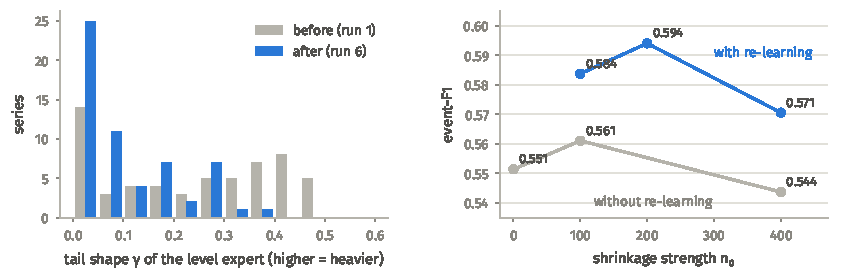
\includegraphics{b_shrinkage}
  \vspace{3mm}
  \begin{columns}[T,onlytextwidth]
    \column{0.48\textwidth}
      {\footnotesize\raggedright \textbf{Left.} Before, the level expert's fitted shape was above 0.3 on 25 of 58
      series: “huge values are normal”, so obvious spikes could not fire. After shrinkage most shapes sit
      near 0 until a series has shown enough extremes to justify a heavy tail.\par}
    \column{0.48\textwidth}
      {\footnotesize\raggedright \textbf{Right.} The strength is bracketed on both sides: 100 and 400 are worse
      than 200. With re-learning the best value moved from 100 to 200, because re-learning absorbs the
      repeat alarms that stronger shrinkage used to cause.\par}
  \end{columns}
\end{frame}

% ------------------------------------------------------------------- B2
\begin{frame}{Backup: re-learning after a regime change}
  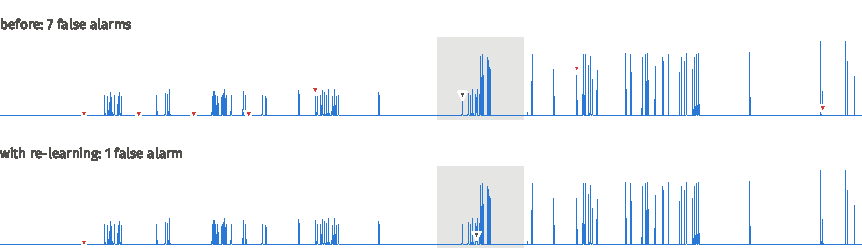
\includegraphics{b_relearn}
  \vspace{3mm}
  \begin{columns}[T,onlytextwidth]
    \column{0.48\textwidth}
      {\footnotesize\raggedright \textbf{The pattern.} A disk sat idle through the warm-up, then started
      working in bursts. The old detector re-fired the moment every 300-point cooldown ended: at points
      461, 762, 1063 and 1364, exactly 301 apart.\par}
    \column{0.48\textwidth}
      {\footnotesize\raggedright \textbf{The rule.} An alarm still on at the first point after the cooldown is
      the same incident, so the normal has changed: rebuild every expert from the last 300 points. Result:
      9 fewer false alarms, no window lost. It fired 3 times in 365,558 points, about 0.2\,s each.\par}
  \end{columns}
\end{frame}

% ------------------------------------------------------------------- B3
\begin{frame}{Backup: what we miss and where false alarms come from}
  \begin{columns}[T,onlytextwidth]
    \column{0.5\textwidth}
      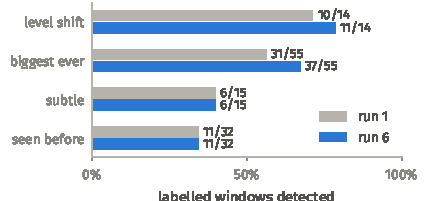
\includegraphics{b_type_rates}
      \figcap{Detection rate by anomaly type, before (run 1) and after (run 6).}
    \column{0.47\textwidth}
      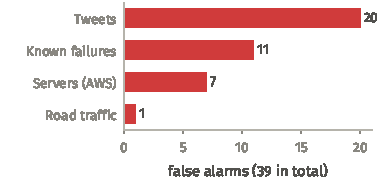
\includegraphics{b_fp_by_category}
      \figcap{The 39 false alarms by category.}
  \end{columns}
  \vspace{4mm}
  {\footnotesize\raggedright The gains are on biggest-ever spikes (31 → 37) and level shifts (10 → 11). “Seen before”
  spikes did not move (11 of 32): an equally big spike already happened unlabelled, so a rarity-based
  detector, by design, has learned that size is normal. Most false alarms are large unlabelled bursts in
  tweet volume.\par}
\end{frame}

% ------------------------------------------------------------------- B4
\begin{frame}{Backup: questions we expect}
  \begin{columns}[T,onlytextwidth]
    \column{0.48\textwidth}
      {\footnotesize\raggedright
      \textbf{Why not deep learning?}\\ Each signal must be learned live from a few hundred points, with
      no training set. Deep models need far more data per signal, adapt slowly and are hard to explain.\\[2.5mm]
      \textbf{Is 0.594 overfitted?}\\ Only global settings, at most 15 runs, and leave-one-category-out
      gives 0.594 too. The ideas were designed on all labels, so expect the hidden test a little lower.\\[2.5mm]
      \textbf{Why is recall 0.56?}\\ 32 of 116 anomalies are “seen before” spikes. On level shifts we find
      79\%, on biggest-ever spikes 67\%.\par}
    \column{0.48\textwidth}
      {\footnotesize\raggedright
      \textbf{What does risk $10^{-5}$ mean?}\\ An alarm fires only when a value is that rare for that
      signal. The same rule holds on every signal; no threshold is set by hand.\\[2.5mm]
      \textbf{Is it really streaming?}\\ Each point is processed once, and the output at time $t$ uses data
      up to $t$ only. Typical cost is 61\,µs per point.\\[2.5mm]
      \textbf{How was the 15-run budget used?}\\ 7 runs: 1 reference, 3 kept, 3 dropped. 7 more ideas were
      rejected from saved outputs without spending a run.\par}
  \end{columns}
\end{frame}

% ------------------------------------------------------------------- B5
\begin{frame}{Backup: why we report event-F1, not point-adjusted F1}
  \begin{columns}[T,onlytextwidth]
    \column{0.40\textwidth}
      \head{Point adjustment, used in many papers}
      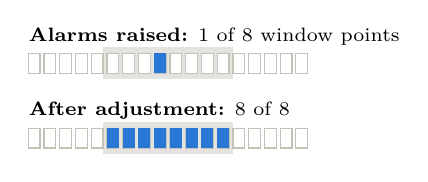
\begin{tikzpicture}[font=\scriptsize, cell/.style={draw=line, fill=white}]
        \foreach \y in {0,-0.95} \fill[winfill] (0.95,\y-0.08) rectangle (2.6,\y+0.33);
        \node[anchor=south west, inner sep=0pt] at (0,0.35) {\textbf{Alarms raised:} 1 of 8 window points};
        \node[anchor=south west, inner sep=0pt] at (0,-0.6) {\textbf{After adjustment:} 8 of 8};
        \foreach \y in {0,-0.95} \foreach \i in {0,...,17} \draw[cell] (\i*0.2,\y) rectangle ++(0.15,0.25);
        \fill[sblue] (1.6,0) rectangle ++(0.15,0.25);
        \foreach \i in {5,...,12} \fill[sblue] (\i*0.2,-0.95) rectangle ++(0.15,0.25);
      \end{tikzpicture}\\[3mm]
      {\footnotesize\raggedright Once any point of a labelled window fires, every point of the window
      counts as found. A median NAB window is 212 points long, so one lucky alarm becomes 212 true
      positives, while each false alarm costs only one point.\par}
    \column{0.56\textwidth}
      {\footnotesize\setlength{\tabcolsep}{4.5pt}
      \begin{tabular}{@{}l r r r@{}}
        \toprule
        & \multicolumn{3}{c}{F1 when scored by}\\
        \cmidrule(l){2-4}
        detector & events & point-adjusted & points\\
        \midrule
        \textbf{\color{sblue}Sentinel (ours)} & \textbf{0.594} & 0.823 & 0.045\\
        random, 1\% of points                 & 0.163 & \textbf{\color{sred}0.919} & 0.018\\
        random, 0.28\% of points              & 0.146 & 0.765 & 0.005\\
        flag every point                      & 0.945 & 0.168 & 0.168\\
        \bottomrule
      \end{tabular}}
      \figcap{Our final labels against detectors that know nothing. 0.28\% is Sentinel's own alarm
              rate. Random rows: mean of 5 seeds. \texttt{python scripts/metric\_check.py}, 0 runs.}
  \end{columns}
  \vfill
  \bandnote{\textbf{Point adjustment rewards noise:} random alarms on 1\% of points beat Sentinel.
    Event-F1, the challenge metric, separates them: random 0.16, Sentinel 0.594. No metric is
    fool-proof: one endless alarm per series touches every window and scores 0.945 on event-F1.
    So we also report the alarm count (106, of which 39 false) and the delay, and keep every alarm short.}
  \vspace{1mm}
\end{frame}

\end{document}
